\documentclass{article}
\usepackage[T1]{fontenc}
\usepackage{lmodern}
\usepackage{graphicx}
\usepackage{amsmath,amssymb}
\usepackage[a4paper,margin=2cm]{geometry}
\usepackage[absolute,overlay]{textpos}
\setlength{\TPHorizModule}{1mm}
\setlength{\TPVertModule}{1mm}
\usepackage[indonesian]{babel}
\usepackage{hyperref}
\setlength{\emergencystretch}{2em}
% unit: Halaman 66

\begin{document}

% === Halaman 66 (llm) ===

\begin{center}
\Large Feistel Network
\end{center}

\vspace{10mm}

\textbf{Encryption:}

\begin{align*}
L_1 &= R_0 & R_1 &= L_0 \oplus f_1(R_0) \\
L_2 &= R_1 & R_2 &= L_1 \oplus f_2(R_1) \\
\dots & & \dots & \\
L_i &= R_{i-1} & R_i &= L_{i-1} \oplus f_i(R_{i-1})
\end{align*}

\vspace{10mm}

\textbf{Decryption:}

\begin{align*}
R_{i-1} &= L_i & L_{i-1} &= R_i \oplus f_i(L_i) \\
\dots & & \dots & \\
R_0 &= L_1; & L_0 &= R_1 \oplus f_1(L_1)
\end{align*}

\vspace{10mm}
Sumber: Cryptography CS 555

% deskripsi: Diagram alir struktur Feistel Network untuk proses enkripsi yang menunjukkan operasi XOR dan fungsi f pada blok L dan R.
% bbox normalisasi: [0.1300, 0.1400, 0.5300, 0.5400]
\begin{textblock*}{84.00mm}(27.30mm,41.58mm)
\noindent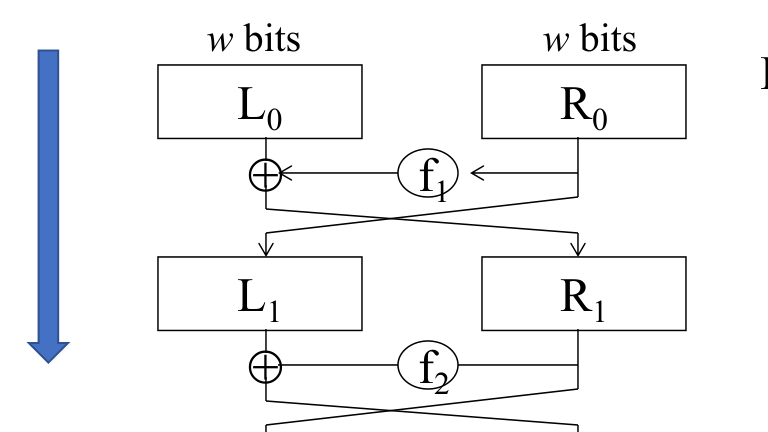
\includegraphics[width=84.00mm,height=118.80mm]{../../images/llm/page_066_img_01.png}%
\end{textblock*}

% deskripsi: Diagram alir struktur Feistel Network untuk proses dekripsi yang menunjukkan pembalikan operasi blok L dan R.
% bbox normalisasi: [0.1200, 0.6700, 0.5300, 0.9200]
\begin{textblock*}{86.10mm}(25.20mm,198.99mm)
\noindent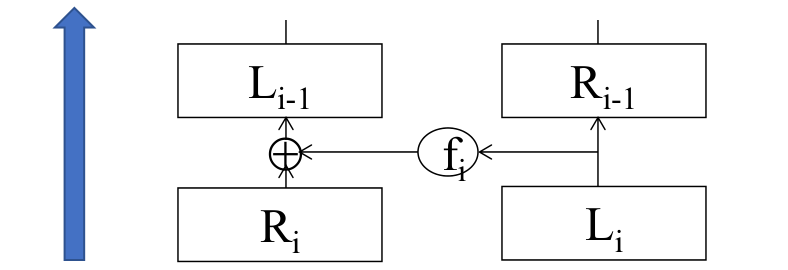
\includegraphics[width=86.10mm,height=74.25mm]{../../images/llm/page_066_img_02.png}%
\end{textblock*}

\end{document}
